%-----------------------------------------------------------------------------%
\chapter{\babDua}
\label{bab:2}
%-----------------------------------------------------------------------------%
Untuk menjawab pertanyaan penelitian yang diuraikan pada Bab~\ref{bab:1}, dibutuhkan dasar pengetahuan yang sesuai. Informasi ini berguna untuk mengetahui potensi pengembangan aplikasi dari berbagai tulisan dan penelitian sebelumnya. Secara umum, bab ini memaparkan mengenai teknologi-teknologi yang terkait dengan pengembangan aplikasi, antara lain WebRTC, CRDT \textit{Conflict-Free Replicated Data Types}, OT (\textit{operational transformation}), dan sifat-sifat pada sebuah editor teks, terutama untuk editor kode. Bab ini juga akan memberikan gambaran mengenai penelitian terkait dan sistem-sistem aplikasi yang sudah pernah dikembangkan sebelumnya. Dalam penelitian ini, terdapat banyak teknologi yang digunakan sebagai media transmisi data, salah satu solusinya dalam aplikasi yang berbasis \textit{client-server} adalah teknologi \textit{websocket}.

\section{WebSocket}

WebSocket merupakan protokol komunikasi dengan kanal dua arah, atau biasa dikenal dengan \textit{full-duplex} yang diinisiasi melalui sebuah koneksi TCP~\citep{fette2011websocket}. Protokol ini bersifat \textit{stateful}, yang berarti koneksi antara klien dan server akan terus bertahan hingga salah satu pihak memutuskan hubungannya~\citep{pimentel2012communicating}. Pada arsitektur perangkat lunak, teknologi ini dapat dimanfaatkan untuk membuat sebuah pola penerbit-pelanggan atau \textit{publisher-subscriber design pattern}~\citep{ganaputra2015asynchronous}. Pada pola ini, klien dapat melakukan permintaan berlangganan ke suatu server dan menjalin hubungan \textit{WebSocket}. Sementara server akan senantiasa memberikan arus data terus menerus setelah adanya pembaharuan kepada setiap klien yang berlangganan. Selain itu, protokol RPC (\textit{Remote Procedure Call}) juga dapat diterapkan di atas \textit{WebSocket}. RPC merupakan istilah pada sistem terdistribusi yang bekerja seperti pemanggilan fungsi pada sebuah \textit{service} atau layanan aplikasi dengan parameter tertentu~\citep{srinivasan1995rpc}. Pada \textit{WebSocket}, setiap pemanggilan \textit{request} RPC menggunakan kanal komunikasi yang sama dan sudah tersedia, sehingga memberikan latensi yang jauh lebih optimal tanpa biaya inisiasi awal tambahan.

WebSocket merupakan teknologi yang sudah ada selama lebih dari 13 tahun saat penelitian ini dilakukan. Berbagai protokol lain kian diteliti untuk mengoptimalkan abstraksi teknologi ini, yaitu dengan mempertahankan fiturnya dan mempercepat performanya. Secara umum, karakteristik WebSocket berbeda dari protokol HTTP atau HTTPS yang bersifat \textit{stateless}. Namun, HTTP/3.0 memberikan potensi protokol baru yang dapat menggantikan WebSocket. Perkembangannya diawali dari HTTP/1.1 yang merupakan salah satu versi protokol HTTP yang dikenalkan pada awal tahun 1997 dan masih digunakan hingga saat ini~\citep{krishnamurthy1999key, fielding2015hypertext}. Pada protokol HTTP/1.1, koneksi TCP yang mendasarinya dapat dipertahankan (\textit{persisted}) dan setiap permintaan atau \textit{request} dikirimkan satu per satu secara berurutan tanpa membuat koneksi baru. Koneksi akan ditutup setelah semua \textit{request} HTTP/1.1 selesai diterima~\citep{fielding2015hypertext}.

Perkembangan HTTP dilanjutkan oleh HTTP/2.0, versi HTTP yang dipublikasikan pada tahun 2015 dan menyediakan fitur \textit{multiplexing}. Setiap \textit{request} pada protokol ini dapat dikirimkan secara paralel dalam suatu koneksi TCP dan membolehkan transmisi data yang lebih efektif ~\citep{belshe2015hypertext}. Secara teori, WebSocket dapat digantikan oleh HTTP/2.0 yang menyediakan \textit{stream} \textit{full-duplex}~\citep{stenberg2014http2}. Namun, \textit{multiplexing} dan persistensi koneksi pada HTTP/2.0 ditujukan bukan sebagai pengganti WebSocket~\citep{fietze2017http}. Versi HTTP/3.0 yang secara teknis berbasis UDP menyediakan API (\textit{application programming interface}) yang dikenal dengan \textit{WebTransport} sebagai alternatif dari \textit{WebSocket} yang lebih optimal~\citep{rfc9114, ietf-webtrans-http3-03}. Hingga waktu penelitian ini dilakukan, protokol \textit{WebTransport} masih dalam pengembangan dan bersifat \textit{draft}. Penggunaannya juga bersifat eksperimental dan terbatas untuk \textit{browser} tertentu~\citep{ietf-webtrans-http3-03}. Teknologi WebSocket digunakan pada layanan yang berbasis \textit{client-server}. Terdapat beberapa protokol lain yang didesain untuk digunakan dalam menghubungkan klien secara langsung atau lebih dikenal dengan arsitektur \textit{peer-to-peer}, salah satunya ialah WebRTC.


\section{WebRTC}

WebRTC merupakan sebuah teknologi web pada browser dan perangkat telepon yang membolehkan koneksi langsung berbasis \textit{peer-to-peer} dalam transmisi datanya~\citep{rfc8835}. WebRTC tidak hanya API (\textit{Application Programming Interface}), namun juga termasuk protokol yang telah didefinisikan pada W3C (World Wide Web Consortium) dan IETF (Internet Engineering Task Force). WebRTC dipublikasikan sebagai teknologi \textit{open-source} oleh Google pada Mei 2011, dan API-nya secara \textit{native} dikembangkan dalam bahasa JavaScript~\citep{dutton2012getting}. Terdapat beberapa komponen dan konsep utama dalam protokol WebRTC, salah satunya ialah komponen jaringan atau koneksinya yang disebut RTCPeerConnection.

Komponen RTCPeerConnection dalam WebRTC merupakan sebuah antarmuka yang merepresentasikan sebuah koneksi antara suatu komputer dan \textit{peer} lainnya dalam suatu jaringan \textit{peer-to-peer}~\citep{rfc8835, rfc8834, jennings2013real}. Dalam sebuah jaringan WebRTC dengan skema \textit{full mesh}, suatu komputer pada sebuah jaringan WebRTC dengan $N$ \textit{peers} akan memiliki $(N-1)$ RTCPeerConnection dengan setiap komputer lainnya dalam jaringan. Terdapat pula skema-skema lain yang mengoptimisasi bentuk jaringan \textit{peer-to-peer} ini dengan keuntungan dan kerugian tertentu.

Penggunaan WebRTC dapat digunakan untuk pertukaran media berupa arus yang didikirimkan terus menerus, sehingga WebRTC menyediakan komponen MediaStream yang merepresentasikan sebuah \textit{stream} atau arus multimedia berupa suara atau video~\citep{sredojev2015webrtc, rfc8835}.~\cite{rfc8830} pada dokumen protokol IETF: \textit{WebRTC MediaStream Identification in the Session Description Protocol} menyampaikan beberapa detail terkait MediaStream pada WebRTC. Sebuah MediaStream dapat mengandung satu atau lebih MediaStreamTrack yang merupakan \textit{track} audio atau video. MediaStreamTrack dapat ditambahkan pada RTCPeerConnection yang nantinya dapat diterima oleh ujung lain dari koneksi tersebut. MediaStream akan menggunakan protokol UDP secara bawaan.

Salah satu komponen lain dalam WebRTC yang signifikan ialah RTCDataChannel yang dijelaskan secara detail pada IETF: \textit{WebRTC Data Channels}~\citep{rfc8831}. RTCDataChannel merupakan kanal data yang digunakan untuk mentransmisikan data apa saja dalam sebuah RTCPeerConnection. Secara teknis, sebuah koneksi dapat memiliki hingga $65534$ RTCDataChannel. Berbeda dengan MediaStream, RTCDataChannel dapat digunakan sebagai kanal untuk membagikan pesan teks atau biner antar klien.

API WebRTC juga menyediakan dua jenis mode pengiriman. Salah satunya ialah mode pengiriman pesan berurutan dan \textit{reliable}, yang konsep pengirimannya sama dengan data yang ditransmisikan dengan protokol TCP (Transmission Control Protocol). Potensi penggunaannya dapat digunakan untuk pengiriman pesan atau berkas. API ini juga menyediakan pengiriman pesan yang tidak harus berurutan dan memperbolehkan kekurangan pesan yang ekuivalen dengan UDP (User Datagram Protocol). Potensi penggunannya bisa untuk permainan, pengendalian perangkat jarak jauh, serta banyak lagi karena memngurangi biaya komputasi \textit{overhead} untuk setiap transmisi datanya, sehingga mode ini bertransmisi dengan lebih cepat. Terakhir, API ini menyediakan pengiriman pesan \textit{partial reliable} dengan protokol SCTP (\textit{Stream Control Transmission Protocol}) yang dapat didefinisikan waktu maksimal \textit{timeout} dan maksimal transmisi ulangnya, urutan dari pesan juga dapat dikonfigurasi.

\subsection{\textit{Signalling Server}}

Sebelum memulai sebuah koneksi antar \textit{peer} dan transmisi media dilakukan, suatu \textit{peer} hendaknya mengetahui informasi semua atau sebagian \textit{peer} lain yang terdapat dalam jaringan tersebut. \textit{Signalling server} bertindak sebagai sebuah server yang mengelola koneksi antar perangkat, namun tidak mengelola lalu lintas media transmisi data itu sendiri~\citep{rfc8839}. server ini hanya sebagai perantara yang memberikan kondisi suatu jaringan dan menandakan \textit{peer} mana saja yang masih terhubung dalam jaringan tersebut. Server akan bertanggungjawab untuk membolehkan sebuah \textit{peer} untuk menemukan \textit{peer} lain di dalam jaringan, mengarahkan pembuatan koneksi untuk \textit{peer} baru yang masuk ke dalam sebuah jaringan WebRTC, serta Mengulang, mematikan, atau melakukan \textit{reset} sebuah koneksi bila diperlukan.

Proses \textit{signalling} ini tidak didefinisikan caranya secara langsung dan memiliki banyak metode alternatif. Terdapat beberapa protokol yang bisa digunakan untuk melakukan \textit{signalling}, antara lain XMPP (Extensible Messaging and Presence Protocol), XHR (XML HTTP Request), dan masih banyak lagi~\citep{sredojev2015webrtc}. Salah satu yang umum digunakan lainnya adalah SIP (Session Initiation Protocol) yang memanfaatkan koneksi \textit{WebSocket} pada setiap klien dengan \textit{signalling server}~\citep{adeyeye2013determining}. Proses \textit{signalling} lebih lanjut didefinisikan menggunakan suatu protokol insiasi yang dikenal dengan SDP (\textit{Session Description Protocol}).

\subsection{SDP (\textit{Session Description Protocol})}
\label{subsec:sdp}

SDP (\textit{Session Description Protocol}) pada dasarnya berisikan informasi-informasi suatu peer kepada peer lainnya.~\cite{rfc8839} menjelaskan secara detail prosedur inisiasi jaringan WebRTC yang menggunakan SDP ini pada dokumen IETF: \textit{Session Description Protocol (SDP) Offer/Answer Procedures for Interactive Connectivity Establishment (ICE)}. Untuk memulai sebuah jaringan, terdapat sebuah objek informasi yang disebut Session Description Protokol yang akan ditawarkan kepada \textit{peer} yang baru masuk ke dalam jaringan WebRTC dan berisi informasi-informasi tertentu mengenai \textit{peer} yang menawarkan tersebut. Misalnya berupa alamat URL, jenis media yang ditransmisikan, \textit{codec}, dan masih banyak lagi. SDP akan dikirimkan kepada signalling server. Setelah \textit{peer} yang ditawarkan menerima, maka \textit{peer} yang ditawarkan tersebut akan memberikan SDP-nya kepada \textit{peer} yang menawarkan, sehingga sebuah jaringan WebRTC akan terjalin. Kandidat yang dapat menerima SDP ini dideskripsikan melalui sebuah ICE Candidate, yaitu sekumpulan rute yang dapat dilalui oleh sebuah \textit{peer} untuk dapat meraih \textit{peer} lain secara langsung. Di dalam SDP, terdapat deskripsi ICE Candidates ini. Dalam beberapa kasus, ICE Candidates akan dikirimkan melalui \textit{signalling server} dengan metode \textit{trickle}, yakni terpisah dari SDP dan ditambahkan satu per satu saat ada ICE Candidate baru yang didapat dari STUN server.

\subsection{ICE (Interactive Connectivity Establishment)}

Dokumen IETF yang diajukan oleh~\cite{rfc8839} juga membahas lebih lanjut mengenai ICE dan mekanisme pencarian alamatnya. Sistem alamat di Internet kebanyakan masih menggunakan protokol IPv4 yang secara praktis tidak dapat memenuhi semua kebutuhan penetapan alamat sehingga setiap perangkat memiliki alamat IP yang berbeda. Perangkat yang digunakan pada suatu jaringan dapat berada di belakang lapisan NAT (\textit{Network Address Translation}). Mekanisme ini memetakan alamat IP Privat menjadi IP Publik atau sebaliknya saat paket data bertransmisi dalam jaringan. NAT pada umumnya diimplementasikan pada sebuah jaringan dalam lingkup kecil, misalnya pada Wi-fi rumah atau instansi tertentu. Pada WebRTC, untuk mengetahui alamat \textit{peer} satu sama lain dibutuhkan suatu protokol yang disebut ICE (Interactive Connectivity Establishment). Server ICE akan mengembalikan ICE Candidate yang mendeskripsikan rute dan protokol yang harus diambil untuk mencapai suatu \textit{peer} tertentu. Terdapat dua jenis server untuk ICE, yaitu STUN (\textit{Session Traversal Utilities for NAT}) and TURN (\textit{Traversal Using Relays around NAT}).

Server STUN merupakan server yang mengembalikan alamat IP publik terhadap \textit{peer} yang menghubungi server itu sendiri, jenis NAT yang digunakan, dan \textit{port} NAT yang diasosiasikan dengan \textit{peer} tersebut. Pengembang dapat menggunakan server STUN publik non komersial, salah satunya milik Google. Apabila koneksi langsung antar-\textit{peer} gagal dilakukan, maka TURN server berguna sebagai server perantara atau \textit{relay server} yang meneruskan koneksi. Hal ini bisa terjadi karena adanya \textit{firewall} yang diletakkan pada bagian mana saja dari jaringan yang memotong hubungan langsung lalu lintas dari WebRTC. TURN merupakan sebuah protokol untuk meneruskan lalu lintas jaringan yang tidak bisa dilakukan secara langsung tersebut. Sebuah TURN server memiliki public IP address yang dapat diakses oleh kedua \textit{peer}, sehingga TURN Server ini dapat bertindak sebagai sebuah jembatan dalam transmisi media antara dua buah \textit{peer} dalam sebuah jaringan WebRTC~\citep{rfc5766}.\newline

Berdasarkan paparan di atas, WebRTC merupakan suatu protokol kompleks yang penggunaannya fleksibel dan berpotensi dalam banyak kasus penggunaan. WebRTC menyediakan jaringan transmisi data secara \textit{peer-to-peer} dengan latensi rendah. Dalam penelitian ini, WebRTC merupakan salah satu teknologi yang dimanfaatkan dalam pengembangan aplikasi. Salah satu komponen lain yang diperlukan sebagai dasar aplikasi ialah pengetahuan mengenai editor kode yang bersifat kolaboratif dan algoritma yang mewujudkannya.

\section{Editor Kode Kolaboratif}

Editor kode merupakan sebuah peralatan atau aplikasi yang digunakan oleh seorang programmer untuk mengembangkan kodenya. Fungsi-fungsi dasar editor kode yang membedakannya dengan editor biasa misalnya sorotan \textit{syntax}, indentasi otomatis, dan penyocokan tanda kurung otomatis~\citep{kinder2013sublime, intellij2011most}. Selain yang disebutkan, masih ada fungsi-fungsi lain yang tidak ada pada editor teks biasa. Dalam penelitian ini, semua operasi yang digunakan dalam editor kode dapat direduksi secara tidak langsung menjadi operasi-operasi pada editor teks biasa (\textit{plain text editor}). Pada \textit{plain text editor}, setiap karakter pada teks tidak mengandung informasi tambahan. Perhatikan ilustrasi pada Gambar~\ref{fig:2:richtext} yang menunjukkan perubahan \textit{styling} yang dapat dilakukan pada \textit{rich text editor}. Operasi semacam ilustrasi tersebut diasumsikan tidak dapat dilakukan pada editor kode karena setiap karakter dianggap tidak menyimpan informasi tambahan.

\begin{figure}
    \centering
    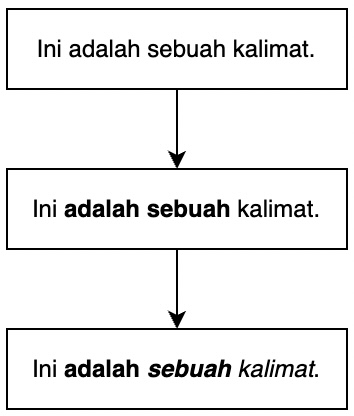
\includegraphics[scale=0.8]{assets/skripsi/richtext}
    \caption{Diagram Contoh Perubahan pada \textit{Rich Text Editor}}
    \label{fig:2:richtext}
\end{figure}

Pada editor kode atau teks yang bersifat kolaboratif setiap pengguna memiliki replikat dari suatu dokumen teks yang akan berakhir sama~\citep{Sun1998, Sun2004}. Setiap pengguna bebas melakukan penyuntingan secara bersamaan tanpa ada larangan tertentu. Operasi lokal kemudian akan diterapkan langsung pada replikat lokalnya tanpa ada jeda~\citep{attiya2016specification, Lv2015}. Operasi yang dilakukan oleh seorang pengguna akan dipropagasi pada setiap pengguna lain secara langsung dengan latensi minimal, sehingga sifat kolaborasi waktu nyata dapat terwujud. Terdapat beberapa algoritma yang akan mewujudkan konsistensi \textit{state} atau keadaan dokumen pada setiap replikatnya. Setiap operasi yang dilakukan oleh setiap pengguna akan menghasilkan dokumen identik yang merupakan hasil penyatuan atau konvergensi yang memenuhi suntingan operasi-operasi tersebut~\citep{Sun1998, Sun2004, Sun2019First, Sun2019third}. Operasi yang dilakukan bersifat komutatif, yang berarti terlepas dari urutan diterapkannya operasi pada suatu dokumen, hasilnya akan tetap sama melalui algoritma yang mewujudkan konsistensi ini~\citep{Sun1998}.

\section{OT (\textit{Operational Transformation})}
\label{subsec:OT}

Salah satu tantangan dalam menciptakan suatu sistem terdistribusi adalah untuk memiliki suatu basis atau struktur data yang nilainya konsisten untuk setiap klien dalam sistem tersebut. Salah satu struktur data yang menjadi fokus penelitian adalah dokumen \textit{plain text}. Metode OT (\textit{Operational Transformation}) dikembangkan dengan motivasi bagi setiap pengguna dalam suatu sistem terdistribusi dapat memiliki dokumen yang sama untuk setiap perubahan yang terjadi~\citep{Sun1998}. Dalam algoritma dasar OT, operasi yang digunakan adalah \texttt{insert(pos, c)}. Operasi tersebut memasukkan sebuah karakter $c$ pada indeks $\texttt{pos}$ dan setiap karakter yang posisi awalnya berada $\geq \texttt{pos}$ akan digeser ke indeks selanjutnya. Ada pula operasi \texttt{delete(pos)} atau menghapus sebuah karakter pada indeks \texttt{pos}~\citep{OTOverview1}. Unit operasi seperti \texttt{insert} dan \texttt{delete} ini merupakan unit dasar dari OT~\citep{OTOverview1}.

OT dibuat untuk menyelesaikan konflik operasi yang dapat terjadi tanpa mengetahui urutan terjadi antar setiap kliennya. OT secara garis besar bekerja melalui sebuah fungsi $T$, yang mentransformasikan dan menyesuaikan parameter suatu operasi $\op$ yang akan dilakukan pada suatu dokumen, berdasarkan operasi-operasi sebelumnya yang telah diterapkan pada dokumen tersebut. Terdapat dua sifat yang umumnya harus dipenuhi oleh suatu algoritma OT untuk bekerja, antara lain sebagai berikut~\citep{crdtLecture, OTOverview1, Li2004, Ressel1996}.

\begin{itemize}
    \item CP1/TP1 (\textit{Convergent Property} 1 atau \textit{Transformation Property} 1), yaitu $\op_1 \circ T(\op_2, \op_1) \equiv \op_2 \circ T(\op_1, \op_2)$.
    \item CP2/TP2 (\textit{Convergent Property} 2 atau \textit{Transformation Property} 2), yaitu $T(\op_{3},\op_{1}\circ T(\op_{2},\op_{1}))=T(\op_{3},\op_{2}\circ T(\op_{1},\op_{2}))$.
\end{itemize}


\begin{figure}[h]
    \centering
    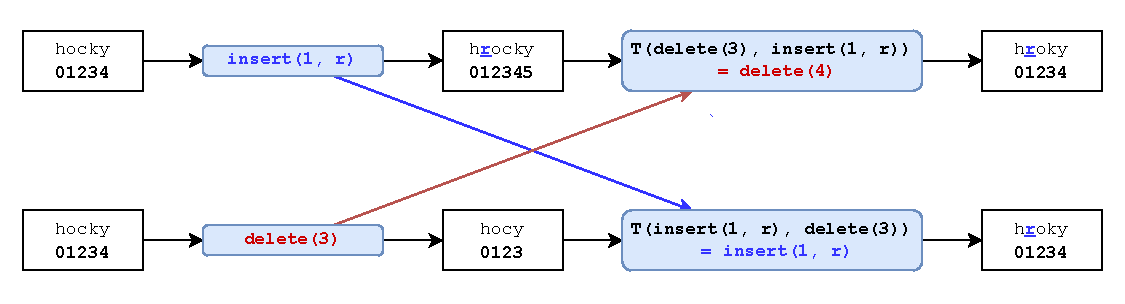
\includegraphics[scale=0.8]{assets/skripsi/OT}
    \caption{Diagram Ilustrasi TP1}
    \label{fig:OTschema}
\end{figure}

TP1 berarti bahwa dokumen yang diterapkan $\op_1$, dan dilanjutkan dengan penerapan operasi tranformasi $\op_2$ terhadap $\op_1$ haruslah ekuivalen dengan dokumen yang diterapkan $\op_2$ dan dilanjutkan dengan penerapan operasi transformasi $\op_1$ terhadap $\op_2$. TP1 diperlukan hanya jika dua operasi yang hendak diterapkan pada suatu replika diterapkan pada urutan yang berbeda. Implementasi algoritma \textit{operational transformation} yang memenuhi properti pertama ini cukup untuk membuat sebuah sistem terdistribusi dengan suatu sumber kebenaran yang berbasis \textit{client-server}. Pada suatu sistem \textit{operational transformation} yang tidak menggunakan TP2, salah satu syarat untuk mencapai konvergensi adalah setiap operasi hanya ditransformasikan pada satu sumber konteks yang sama~\citep{Xu2016}. Misalnya riwayat setiap operasi-operasi yang terdapat pada server dianggap sumber operasi yang mutlak untuk setiap klien~\citep{Vidot2000}. Saat klien menerima pembaharuan operasi, semua operasi lokal pada klien yang belum ditambahkan pada server akan ditransformasikan berdasarkan milik server. Operasi dari klien baru bisa di-\textit{append} ke server jika semua operasi yang terdapat pada server sudah dimiliki klien.

Properti lainnya yang harus dimiliki oleh \textit{operational transformation} ialah TP2 yang mengimplikasikan bahwa untuk tiga operasi berbeda, suatu operasi $\op_3$ yang ditransformasikan terhadap dua operasi yang sudah diterapkan lainnya, yaitu $\op_1$ dan $\op_2$ dengan sembarang urutan akan menghasilkan hasil transformasi yang sama. TP2 hanya dibutuhkan untuk sistem yang yang mengizinkan kedua operasi dijalankan pada dua \textit{state} dokumen yang berbeda. Berbeda halnya dengan TP1, \textit{update} secara \textit{concurrent} dapat terjadi untuk klien yang berbeda. Karena kerumitan algoritmanya dan beberapa penelitian dibuktikan salah dalam mengimplementasikan OT yang memenuhi TP2~\citep{OTOverview1}, CRDT dikenalkan sebagai alternatif dari OT sebagai metode untuk menjaga konsistensi dan kebenaran dari suatu dokumen atau data dalam sebuah jaringan sistem terdistribusi.

\section{CRDT (\textit{Conflict-Free Replicated Data Type})}

Sekitar awal tahun 2006, algoritma WOOT (\textit{WithOut Operational Transformation}) yang diteliti oleh~\cite{oster2005real} dikenalkan sebagai sebuah algoritma non-OT pertama untuk memastikan sifat konvergen dari replika teks pada editor kolaboratif sebagai alternatif dari OT. Tidak hanya itu, konsistensi dari \textit{intention} atau maksud dari sebuah operasi juga dapat dijaga~\citep{Li2004}. Misalnya ketika sebuah klien memasukkan sebuah karakter \texttt{X} di antara dua buah karakter \texttt{A} dan \texttt{B} pada sebuah \textit{string} dengan penomoran indeks dari $0$, ``\texttt{ABCDE}''. Operasi yang menjaga \textit{intention}, memiliki makna bahwa masukkan karakter \texttt{X}, sehingga \texttt{A} mendahului \texttt{X} dan \texttt{X} mendahului \texttt{B}. Dengan kata lain, operasi \texttt{insert} yang direpresentasikan sebagai operasi $\texttt{insert}(1, \texttt{X})$ pada OT, direpresentasikan sebagai operasi $\texttt{insert}(\texttt{A} \prec \texttt{X} \prec \texttt{B})$ pada algoritma ini. Dengan \texttt{A} dan \texttt{B} merupakan suatu objek yang memiliki ID pengenal yang bersifat unik untuk setiap karakter yang ada di dalam \textit{string}. Algoritma ini menjadi awal dari perkembangan struktur data CRDT yang secara formal didefinisikan untuk tidak hanya pada \textit{string}, namun berbagai struktur data abstrak lain pada tahun 2011 oleh~\cite{Shapiro2011}.

CRDT sendiri merupakan suatu tipe data abstrak untuk memelihara kecocokan dokumen pada beberapa replikanya dalam sebuah jaringan. Tipe data abstrak berarti semantiknya didefinisikan dari kumpulan nilai properti dan operasi fungsi atau prosedur. Oleh karena itu, implementasi dari CRDT untuk setiap operasinya bisa berbeda-beda, tapi menghasilkan \textit{behavior} yang sama untuk operasi yang sudah didefinisikan. CRDT didesain untuk disimpan pada setiap node atau \textit{peer} dalam sebuah jaringan. Oleh karena itu, implementasi CRDT yang efisien terhadap memori dan waktu juga menjadi pertimbangan dalam menggunakan struktur data ini. Struktur data ini memiliki karakteristik pada setiap replikanya yang bisa dimodifikasi tanpa berkoordinasi dengan replika lain, bila setiap replika dilakukan operasi yang sama tanpa memerhatikan urutannya, maka semuanya akan menghasilkan \textit{state} atau keadaan akhir yang sama~\citep{Shapiro2011, CRDToverview2}.

Salah satu dari contoh CRDT yang sederhana ialah \textit{unordered set} atau himpunan tak berurut~\citep{Shapiro2011}. Pada tipe data tersebut, setiap \textit{peer} dapat melakukan operasi \texttt{insert(v)}, yaitu menambahkan suatu elemen \texttt{v} ke dalam \textit{set} atau himpunan. Selanjutnya, ada pula operasi \texttt{erase(v)} yang akan menghapus elemen \texttt{v} dalam himpunan bila ada. Dalam penelitian ini, tipe data CRDT digunakan dalam proses pengolahan teks, sehingga operasi-operasi yang terkait dengan CRDT yakni serupa dengan yang disampaikan dengan operasi pada bagian~\ref{subsec:OT}, yakni \texttt{insert(pos, c)} serta \texttt{delete(pos)}.

Pada CRDT untuk teks biasa, setiap karakter akan memiliki ID berbeda. Saat melakukan operasi \texttt{insert}, data perubahan akan disertai dengan dua ID referensi karakter sebelum dan sesudahnya serta sebuah \textit{logical clock} untuk menandai urutan pemasukan karakter, seperti ide serupa yang disampaikan pada bagian awal subbab ini~\citep{oster2005real}. Terdapat beberapa cara yang umum diterapkan untuk merepresentasikan CRDT dan menangani kasus \textit{operasi} \texttt{delete}. Cara pertama ialah dengan menyimpan karakter yang sudah dihapus pada suatu dokumen selamanya, dan hanya akan ditandai sebagai ``terhapus'' teknik ini dikenal dengan istilah \textit{tombstone}~\citep{molli2006tombstone}. Pendekatan yang lainnya ialah dengan memberikan ID yang sudah terurut sesuai dengan urutan posisinya. Saat melakukan operasi \texttt{insert} pada suatu posisi tertentu, ID-nya akan lebih besar daripada ID karakter sebelumnya dan lebih kecil daripada ID sesudahnya. ID ini hendaknya bersifat dinamis dan ukurannya dapat bertambah seiring dengan bertambahnya karakter. Setiap ID disertai dengan pengenal tambahan berbeda untuk setiap kliennya yang memastikan ID-nya tidak ada yang duplikat. Saat melakukan operasi \texttt{delete}, node yang hendak dihapus tidak perlu disimpan pada suatu dokumen selamanya karena properti dari urutan ID ini.

Bila dibandingkan dengan OT yang hanya memanfaatkan fungsi transformasi operasi dan dokumennya direpresentasikan secara minimal sebagai \textit{array} karakter saja, CRDT membutuhkan struktur data tambahan untuk setiap karakter pada dokumen. Karakter tersebut akan diberikan ID dan dikenalkan sebagai objek. Karakter tersebut juga akan memiliki urutan penghubung (implisit maupun eksplisit) seperti yang disampaikan pada dua pendekatan CRDT di atas yang menyatakan urutan karakter sebelum dan sesudahnya. Terdapat pula perbedaan-perbedaan lainnya yang dijelaskan lebih lanjut pada subbab~\ref{sec:perbandingan} selanjutnya.

\section{Perbandingan Lanjut CRDT dan OT}
\label{sec:perbandingan}

Industri teks editor kolaboratif waktu nyata masih didominasi oleh \textit{operational transformation} meskipun CRDT memiliki kompleksitas dan efisiensi yang diklaim lebih optimal dibandingkan OT~\citep{Sun2019third}. Tidak ada definisi perbedaan yang terlalu jelas untuk kapan suatu algoritma menggunakan OT dan CRDT, karena pada dasarnya keduanya merupakan transformasi untuk mencapai komutativitas dari fungsi yang direalisasikan menggunakan parameter yang berbeda. Pada CRDT, operasi diubah menjadi representasi ID atau tanda pengenal lain, kemudian dikembalikan ke bentuk posisinya lagi setelah diaplikasikan, sementara pada OT, operasi dinyatakan dengan posisi dari karakternya langsung.

Pendekatan \textit{operational transformation} berlangsung dan terfokus pada algoritma transformasi fungsi yang mengelola dan mengendalikan operasi dari setiap kliennya yang berlangsung bersamaan. Sementara CRDT terfokus pada konten seperti urutan objek, operasi yang berbasis \textit{identifier} atau ID pengenal, dan skema atau representasi lain dalam menyatakan operasi penyuntingan~\citep{Sun2019Second, Sun2019First}. Hal ini membuat struktur data CRDT lebih spesifik penggunaannya untuk tipe data abstrak tertentu, misalnya untuk \textit{set}, \textit{map}, dan teks memiliki implementasi dan algoritmanya masing-masing. Perbedaan pendekatan ini menyebabkan kompleksitas dari kedua metode ini berbeda. Pada OT, variabel kompleksitas dipengaruhi oleh banyaknya operasi yang berlangsung secara bersamaan, dan tidak ada biaya untuk merepresentasikan dan memanipulasi karakter pada teks ke dalam bentuk objek dan struktur datanya. Pada CRDT, variabel kompleksitas ini akan semakin besar dan berbanding lurus dengan ukuran dokumen atau banyaknya konten. Selain itu, biaya \textit{overhead} kompleksitas waktu dan memori inisialisasi untuk \textit{peer} baru yang masuk ke dalam jaringan juga cenderung lebih besar dibandingkan OT.

Bila dilihat dari pembuktian dari kebenaran algoritmanya, CRDT memiliki kerumitan yang lebih tinggi dibandingkan OT karena adanya perlakuan khusus terhadap \textit{state} kontennya~\citep{Sun2019Second}. Terdapat banyak sekali variasi algoritma dari CRDT, sehingga pembuktian sifat konvergennya cenderung lebih sulit dibandingkan OT yang kriteria kebenarannya properti-properti khusus yang sudah dibuktikan pada penelitian-penelitian sebelumnya~\citep{OTOverview1, Sun2004, oster2005real}. Berdasarkan penelitian~\cite{Sun2019Second}, kompleksitas waktu yang diperlukan untuk sistem OT yang merupakan {state-of-the-art} saat ini dalam mengaplikasikan operasi \textit{remote} adalah $O(c)$ dan operasi lokal ialah $O(1)$, dan kompleksitas memori $O(c)$ atau $O(c \cdot m)$ dengan $c$ adalah banyaknya banyaknya operasi bersamaan yang akan ditransformasikan (dalam praktisnya nilainya sangat kecil $(c \leq 10)$ karena operasi berlangsung dalam waktu nyata) dan $m$ adalah banyaknya pengguna dalam jaringan (umumnya $m \leq 5$). Sementara pada CRDT, definisikan $C$ sebagai ukuran konten (tanpa \textit{tombstone}) dan $C_t$ sebagai konten seumur dokumen (dengan \textit{tombstone}). Kompleksitas waktu untuk setiap operasinya dapat berkisar antara $O(C_{t}^{2})$, $O(C_{t})$, hingga $O(1)$ untuk CRDT berbasis \textit{tombstone}, dan $O(\log C)$ untuk solusi yang tidak berbasis \textit{tombstone}. Sementara kompleksitas optimal memorinya bisa mencapai $O(C)$ untuk solusi berbasis \textit{non-tombstone} dan \textit{tombstone} dengan \textit{garbage-collection}. Nilai dari $C$ umumnya berkisar antara $10^3 \leq C \leq 10^6$ untuk dokumen biasa pada umumnya. Implementasi dari CRDT dan variasinya dibahas lebih lanjut pada subbab~\ref{sec:penelitian_terkait}.

\section{Penelitian Terkait}
\label{sec:penelitian_terkait}

Penelitian ini menggunakan \textit{library} Yjs yang mengimplementasikan algoritma YATA (\textit{Yet Another Transformation Approach}) untuk CRDT-nya. YATA menggunakan \textit{linked-list} dalam merepresentasikan datanya dan menggunakan sistem \textit{tombstone} dengan proses \textit{garbage-collector} dalam mengoptimisasi objek konten yang dinyatakan terhapus. Dalam algoritma YATA yang diteliti oleh~\cite{Nicolaescu2016yjs}, operasi \texttt{insert} dinyatakan sebagai menambahkan sebuah objek $o(id, left, right, isDeleted, content)$ ke \textit{linked-list}. Tanda pengenal $id$ berisikan pasangan berurut ID \textit{peer} dan \textit{logical timestamp} berupa operasi ke berapa yang telah dilakukan \textit{peer} tersebut. Properti $left$ dan $right$ masing-masing merupakan variabel yang menandakan $id$ untuk objek yang berada di sebelah kiri dan kanannya saat operasi \texttt{insert}. Bagi teks editor untuk mengetahui keberadaan objek tersebut, terdapat properti $isDeleted$ yang merupakan nilai \textit{boolean} yang menunjukkan sudah terhapus atau tidaknya objek tersebut, serta properti $content$ yang merupakan \textit{string} yang berisi konten data dari objek tersebut.

Optimisasi pada Yjs terdapat pada properti $content$ yang dapat berupa \textit{string} atau kumpulan karakter. Saat ada operasi \texttt{insert} di antara dua konten dalam objek yang sama, objek tersebut akan dibagi menjadi dua objek lain. Sehingga dalam representasinya, \textit{logical timestamp} juga akan menyimpan informasi panjang konten di objek saat ini. Operasi penghapusan dilakukan dengan secara sederhana menandai objek tersebut menjadi terhapus. Untuk detail implementasi dan kompresi lebih lanjut disampaikan pada penelitian YATA~\citep{Nicolaescu2016yjs}.

Yjs merupakan \textit{library} yang baru populer digunakan pada tiga tahun terakhir selama penelitian ini. Terdapat beberapa implementasi algoritma lain seperti Logoot yang menggunakan \textit{vector clock} pada \textit{timestamp} objeknya. \textit{Vector clock} atau \textit{state vector} secara sederhana merupakan sebuah vektor yang merepresentasikan versi dari setiap \textit{peer} dalam jaringan. Dalam Logoot, operasi penghapusan dilakukan langsung dengan menghapus objek tanpa perlu menyimpan \textit{tombstone}~\citep{weiss2009logoot}.

CRDT YATA melanjutkan ide awal dari CRDT LSeq (Linear Sequences) yang ID pengenalnya tidak menggunakan \textit{timestamp}. Permasalahan dari algoritma ini ialah dapat terjadinya \textit{interleaving}, yakni urutan untuk operasi \texttt{insert} yang dilakukan bersamaan tidak memiliki komparator lanjutan (hanya \textit{partial order}) saat adanya konkurensi yang terjadi ketika terdapat lebih dari satu karakter memiliki penunjuk objek \textit{left} dan \textit{right} sama pada dua \textit{peer} berbeda~\citep{kleppmann2019interleaving, nedelec2013lseq}. YATA menyelesaikan masalah ini dengan menambahkan \textit{logical timestamp} untuk setiap kliennya.

Alternatif dari YATA, yaitu RGA (Replicated Growable Array) menyelesaikan masalah \textit{interleaving} pada LSeq dengan menggunakan pasangan berurut ID \textit{peer} dan \textit{timestamp global} yang didapat dari \textit{timestamp} selanjutnya dari \textit{timestamp} operasi terkecil pada CRDT. Dalam praktisnya, algoritma ini memiliki berbagai optimisasi lebih terlepas dari algoritma yang disampaikan pada penelitian formalnya. Misalnya penambahan \textit{garbage collector}, kompresi data antar jaringan, dan penyimpanan objek dalam memori yang memengaruhi performanya.